
\documentclass[preprint,12pt]{elsarticle}

%This version has suggestions of Tamas, Veera and Stephen
\usepackage{graphics}
\usepackage{amssymb}
\usepackage{lineno}
\usepackage{url}

\usepackage{lineno}
\usepackage{url}
\usepackage{color}
\usepackage{soul}

%% Commands
\newtheorem{definition}{Definition}
\biboptions{comma,square}


\newcommand{\hlc}[2][yellow]{ {\sethlcolor{#1} \hl{#2}} }
\newcommand{\Tamas}[1]{{\color{red}#1}}
%\newcommand{\edson}[1]{{\color{red}#1}}
\newcommand{\paulo}[1]{{\hlc[cyan]{\textbf{Paulo}: #1}}}
\newcommand{\Tcomment}[1]{{\color{red}#1}}
%\newcommand{\marcos}[1]{{\color{green}#1}}

\newcommand{\sandro}[1]{\hl{Sandro: #1}}
\newcommand{\joel}[1]{{\hlc[green]{\textbf{Joel}: #1}}}

\newcommand{\qm}[1]{``#1''}

\journal{Robotics and Computer-Integrated Manufacturing}

\begin{document}

\begin{frontmatter}

%% Title, authors and addresses

%% use the tnoteref command within \title for footnotes;
%% use the tnotetext command for the associated footnote;
%% use the fnref command within \author or \address for footnotes;
%% use the fntext command for the associated footnote;
%% use the corref command within \author for corresponding author footnotes;
%% use the cortext command for the associated footnote;
%% use the ead command for the email address,
%% and the form \ead[url] for the home page:
%%
%% \title{Title\tnoteref{label1}}
%% \tnotetext[label1]{}
%% \author{Name\corref{cor1}\fnref{label2}}
%% \ead{email address}
%% \ead[url]{home page}
%% \fntext[label2]{}
%% \cortext[cor1]{}
%% \address{Address\fnref{label3}}
%% \fntext[label3]{}

\title{Extensions to the Core Ontology for Robotics and Automation}


\author[ufrgs]{Sandro Rama Fiorini\corref{cor1}}
\ead{srfiorini@inf.ufrgs.br}

\author[ufrgs]{Joel Luis Carbonera}
\ead{jlcarbonera@inf.ufrgs.br}

\author[paulo1,paulo2]{Paulo Gon\c calves}
\ead{paulo.goncalves@ipcb.pt}

\author[ufrgs]{Vitor A. M. Jorge}
\ead{vamjorge@inf.ufrgs.br}

\author[ufrgs]{V\'itor Fortes Rey}
\ead{vfrey@inf.ufrgs.br}

\author[tamas1,tamas2]{Tam\'as Haidegger}
\ead{haidegger@ieee.org}

\author[ufrgs]{Mara Abel}
\ead{marabel@inf.ufrgs.br}

\author[signe]{Signe A. Redfield}
\ead{signe@ieee.org}

\author[stephen]{Stephen Balakirsky}
\ead{stephen.balakirsky@gtri.gatech.edu}

\author[veera]{Veera Ragavan}
\ead{veera.ragavan@monash.edu}

\author[howard]{Howard Li}
\ead{vhoward@unb.ca}

\author[craig]{Craig Schlenoff}
\ead{craig.schlenoff@nist.gov}

\author[ufrgs]{Edson Prestes}
\ead{edson.prestes@ieee.org}

\address[ufrgs]{Instituto de Inform{\'a}tica, UFRGS, Brazil}

\address[paulo1]{Polytechnic Institute of Castelo Branco, School of Technology, Portugal}

\address[paulo2]{LAETA, IDMEC, Instituto Superior T{\'e}cnico, Universidade de Lisboa, Lisboa, Portugal}

\address[tamas1]{\'Obuda University, Budapest, Hungary}

\address[tamas2]{Austrian Center for Medical Innovation and Technology (ACMIT), Wiener Neustadt, Austria}

\address[signe]{Naval Research Laboratory, USA}

\address[stephen]{Robotics and Autonomous Systems Division, Georgia Tech Research Institute, USA}

\address[veera]{School of Engineering, Monash University, Sunway Campus, Malaysia}

\address[howard]{Dept. of Electrical and Computer Engineering, University of New Brunswick, Canada}

\address[craig]{Intelligent Systems Division, NIST, USA}

\cortext[cor1]{Corresponding author}




\begin{abstract}
The working group \emph{Ontologies for Robotics and Automation}, sponsored by the \emph{IEEE Robotics \& Automation Society}, recently proposed a Core Ontology for Robotics and Automation (CORA). This ontology was developed to provide an unambiguous definition of core notions of robotics and related topics. It is based on SUMO, a top-level ontology of general concepts, and on ISO 8373:2012 standard, developed by the ISO/TC184/SC2 Working Group, which defines --- in natural language --- important terms in the domain of Robotics and Automation (R\&A). In this paper, we introduce a set of ontologies that complement CORA with notions such as industrial design and positioning. We also introduce updates to CORA in order to provide more ontologically sound representations of autonomy and of robot parts. 

%\joel{We need to rewrite the abstract}
%\sandro{Done. Check, please!}

\end{abstract}

\begin{keyword}
Ontologies for robotics and automation \sep Ontology-based standards \sep  Core ontology \sep Ontology engineering \sep Knowledge representation.
\end{keyword}
\end{frontmatter}

%\linenumbers

\section{Introduction}



%Communication and reasoning about robots and related notions requires a well-structured \textit{body of knowledge} about robots. This is a crucial requirement for unambiguous communication and reasoning for robots, and also important for sharing information about robots among humans.
A well-structured \emph{body of knowledge} for robotics and automation (R\&A) is a crucial requirement not only for unambiguous communication and reasoning for robots, but also for knowledge and information sharing about robots among humans and for interaction between robots and humans. Recently, such bodies of knowledge have been successfully developed using ontologies. Ontologies are information artifacts that specify in a \emph{formal} and \emph{explicit} way the domain knowledge \emph{shared} by a community \cite{STUDER1998}. The availability of well-founded methodologies allow us to develop ontologies in a principled way. The artifacts that result from this process ensure mutual agreement among stakeholders, increase the potential for reuse of the knowledge, and promote data integration.
%The general methodology for building ontologies specify certain modelling principles that must be followed in order to assure that the finished artifact commits to the shared knowledge, ensuring the mutual agreement among stakeholders, and increasing the potential of reuse of the knowledge, allowing  data integration. 

In order to specify and clarify the meaning of the core notions common in R\&A, the Working Group (WG) \emph{Ontologies for Robotics and Automation} (ORA), sponsored by the \emph{IEEE Robotics \& Automation Society}, have proposed a \emph{Core Ontology for Robotics and Automation} (\emph{CORA}). This ontology is meant to be used by robots and roboticists in tasks that require explicit knowledge about robots, such as robot-robot and robot-human communication, robot design, and integration of data about robots. The aim of the ORA WG is to standardize knowledge representation in the R\&A field \cite{schlenoff2012ieee}. Within this broad context, CORA is intended to provide the core conceptual structure that will integrate other specific ontologies developed for the domain of R\&A. 

CORA has been developed taking into account theories of the discipline of Formal Ontology \cite{Guizzardi2005}. In particular, many of our ontological choices were evaluated based on guidelines from known methodologies, such as METHONTOLOGY \cite{Fernandez97} and OntoClean \cite{Guarino2009}. Besides that, CORA was developed based on SUMO \cite{SUMO}; a top-level ontology that aims to define the main ontological categories describing the world. Such an approach is new in developing standards in R\&A and has the advantage of producing a better founded standard, which requires less work to use, maintain and extend.

This work reports the recent developments within the ongoing CORA project, and provides an overview of its current state. The prior version of CORA \cite{prestes2013towards} has been extended, implementing changes in modeling decisions and introducing new concepts and relations. Thus, this paper presents some changes in modelling decisions that have been implemented since the previous version. The major new contributions can be divided into two broad areas. First, we propose CORAX, an ontology that covers concepts  too general to be part of CORA, and that are not covered by SUMO. These  include knowledge about \emph{design} (as in the case of product design), \emph{physical environment}, \emph{interaction}, and \emph{artificial systems}. Second, we propose extensions and changes to CORA itself, in order to improve its ontological commitment to the domain. We are primarily concerned with representation of \emph{operation modes} and \emph{robot parts}. Finally, we discuss some directions regarding new, yet to be covered topics (such as control and planning).

%\joel{The section The IEEE RAS working group was removed?}
%\section{Preliminaries: Ontology Engineering}

%\subsection{Steps to build the ontology}
%\joel{A shortened (and abstracted) version of the methodology section in our RAS paper?}

%\subsection{The IEEE RAS working group}

%\textbf{same text as previous RAS paper, must be changed to the actual state}

%The \emph{IEEE RAS Ontologies for Robotics and Automation Working Group} (ORA WG) was created in 2011 with the aim to link existing ISO, IEC, etc.~standards and the current research efforts towards new regulatory frameworks~\cite{HF5}. The goal is to develop a standard for knowledge representation and reasoning in robotics and automation, together with the representation of concepts of an initial set of application domains~\cite{schlenoff2012ieee}.

%The ORA WG  is comprised of over 50 members, representing over twenty countries, a cross-section of industry, academia and government. The group has four years to prepare a document that will be evaluated by invited experts, organizations and the \emph{IEEE--SA Standards Board}. The ORA WG is composed of four sub-groups. Three sub-groups are in charge of developing ontologies for three subdomains of R\&A: industrial robotics, service robotics, and autonomous robotics. The fourth subgroup, called Upper Ontology/Methodology (UpOM), works in the development of a more general ontology that will bring all of the subdomain ontologies together. CORA is the main result of the efforts performed by UpOM.
%There are four sub-groups, of which one is dedicated to \emph{service robotics}~(SeR).
%\joel{Why emphasising the service robotics group?}
%The SeR group is developing ontologies, by defining service robotic concepts and the relationship among concepts such that humans and robots can interact to perform tasks in any environment. These ontologies will be used for reasoning by robots to perform tasks.
%The ontologies developed by the ORA WG are intended to be merged in a broad ontology that can be further extended for cover specific applications in R\&A. The final ontology will ensure a common understanding among members of the community and facilitating more efficient integration and data transfer. 

%\joel{I think that the content below fitts better the next section. There is an overlap.}
%This is guaranteed through the ontology engineering process used that removes ambiguities and wrong relationships. ORA WG uses two methods called METHONTOLOGY~\cite{Fernandez97} and OntoClean~\cite{Guarino2009}. METHONTOLOGY is for building ontologies either from scratch, by reusing other ontologies, or by re-engineering existing ones. It has a check list that allows for the identification of inconsistencies, incompleteness and redundancy. On the other hand, OntoClean helps to validate the ontology according to ontological adequacy of taxonomic relationships. It is based on general ontological notions drawn from philosophy, like essence, identity, and unity.

%Furthermore, the ORA ontology is described through mathematical formalism where each concept and relationship is well-grounded mathematically, using logics. In this case, the group uses description logics expressed in OWL. OWL is  used due to popularity in the ontology development community, and due to the number of tools and reasoning engines available. Moreover, it provides additional vocabulary, and facilitates greater machine interoperability of web contents. In this sense, the ORA ontology will be available to the R\&A community to be used as a knowledge source for various applications.
%\joel{axiomatization in SUO-KIF and implementation in OWL?}

%\emph{Tell something about our interest in ontology development. What is our real goal?}

%The objective of this ontology development effort is to identify, develop, and document the salient terms and their definitions so that they can serve as a common reference for the R\&A community.
%The goal of the work group is also to coordinate the standardization efforts with other groups to facilitate more effective information sharing, while achieving wider impact.
%An important issue towards a united service robot ontology is the implementation of it, determined by its modularity, reusability and flexibility. The ORA WG decided to use\emph{Ontology Web Language} (OWL) because of its popularity among the ontology development community, and for the number of tools and reasoning engines that are available. Besides, it provides additional vocabulary, and facilitates greater machine interoperability of Web content.

%In practice, the ontologies from each group (AuR, SeR, InD) are being developed collaboratively in a web tool called WebProt\`eg\`e
%\footnote{WebProt\`eg\`e~\cite{webprotege} from  \emph{Stanford University School of Medicine} is based on the worldwide used ontology editor Prot\`eg\`e, having nearly 200,000 users. It is a free and open-source platform that provides a suite of tools to create domain model and knowledge base application using ontologies.}
%that allows sub-group members to hold discussions, and edit the ontologies on-line \edson{Is that correct? Who is using web protege?}.
%Prot\`eg\`e will be used more extensively in the final stage of the process, after having sent an open call to the overall robotics community for contribution to an easy-to-use wiki environment. The wiki architecture was chosen because it is a widely used, actively maintained open-source platform that supports highly efficient reasoning like \emph{Semantic Web Rule Language} (SWRL)~\cite{OConnor2005}.

%In the next phase, the sub-group chairs will invite well-known experts of the field to review each step of the process and have a suitable and consensual ontology. Meanwhile, the other sub-groups of the ORA WG are concurrently developing their ontologies. After each round of expert review, the Upper Ontology sub-group will update the ontologies that can be merged and used by all.

%In service robotics, the environment, i.e., context space~\cite{Hallam_Bruyninckx_2006} is a key factor, since the ontologies for this kind of robots must ``fit'' a large number of scenarios and application areas.  It must be modular and reusable between scenarios and applications. The application fields identified by the \emph{IEEE RAS Technical Committee on Service Robots}~\cite{ieee_ras_tc_ser} are used by this group. The different concepts within the ontology will all receive the input from the other subgroups to produce a consensual, common list for the robotics community at large.

%\subsection{Example of ontological application in health care}
% moved


%\section{Application-oriented development}
%moved.


\section{Ontology Engineering}


We developed CORA using several ontology tools and frameworks. The main methodology is based on METHONTOLOGY \cite{Fernandez97}, which provides a methodology for building ontologies either from scratch, by reuse, or by re-engineering existing ones. In general, it consists of a set of guidelines about how to carry out the activities identified in the ontology development process, the kinds of techniques that are the most appropriate for each activity, and the resulting products. 

We also based many of the underlying \textit{ontological commitments} on \textit{OntoClean} \cite{Guarino2009}. Ontoclean is a methodology for validating the ontological adequacy of taxonomic relationships, based on highly generic ontological notions drawn from philosophy, like \textit{essence}, \textit{identity} and \textit{unity}. These notions are used to characterize relevant aspects of the intended meaning of the properties, classes, and relations that compose an ontology. OntoClean requires the ontology engineer to explicitly identify the ontological commitments underlying the concepts that are being modelled. As a result, OntoClean allowed us to identify ambiguities in the definitions of core notions provided by other standards of R\&A (see \cite{prestes2013towards} for more details).

In addition, as a result of an evaluation process carried out in \cite{prestes2013towards}, we selected the \emph{Suggested Upper Merged Ontology} (SUMO)\footnote{\url{http://www.ontologyportal.org/}} \cite{SUMO} as the most suitable top-level ontology for supporting the development of CORA. SUMO was developed by an IEEE working group, and according to our analysis, it is flexible enough to fit the purposes of the project. It includes the main notions and distinctions we would like to introduce in our ontology, such as \textit{agent}, \textit{device} and \textit{agent group}. All concepts in CORA and related ontologies are specializations of concepts in SUMO. 

SUMO defines the  basic ontological categories across all domains. The remainder of this section gives a brief overview of its main concepts, illustrated in Fig.~\ref{fig:sumo}. Detailed information can be found in \cite{SUMO}. 
 
\begin{figure}[th] 
	\centering  
	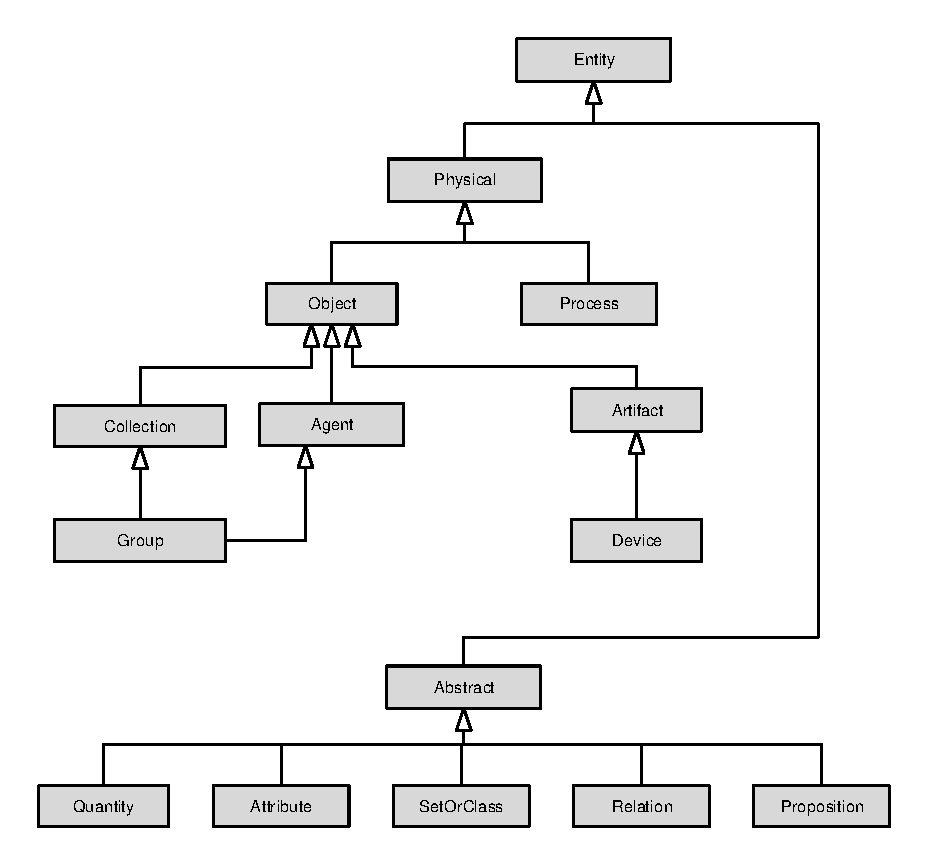
\includegraphics[width=0.9\textwidth]{figs/sumo}  
	\caption{Overview of top-level concepts of SUMO.}  
	\label{fig:sumo}  
\end{figure}  


The main SUMO category is \emph{Entity}, which is a disjoint partition of \emph{Physical} and \emph{Abstract} entities. Physical represents entities that have a location in space-time. Abstract describes entities that do not have a location in space-time.

Physical is further partitioned into \textit{Object} and \textit{Process}. Object exists in space, keeping its identity in time, and has spatial parts but not temporal parts. Process is the class of instances that happen in time and have temporal parts or stages. This means SUMO follows an \emph{endurantist} perspective instead of a \emph{perdurantist} one. For a perdurantist, an object is composed by every temporal part it has at all times. On the other hand, for an endurantist, an object changes through time, but keeps the essential parts that define its identity. A good analogy is to think that perdurantists see objects as tunnel-like regions in a 4D space, while endurantists see them as a 3D region that travels through the time dimension.

Abstract is further partitioned into \textit{Quantity, Attribute, SetOrClass, Relation} and \textit{Proposition}. Quantity abstracts numeric and physical quantities. Attribute abstracts qualities that cannot or are chosen not to be considered as subclasses of Object. SetOrClass abstracts entities that have \emph{elements} (in the case of sets) or \emph{instances} (in the case of classes). Relation generalizes n-ary relations, functions and lists. Finally, Propositions are entities that express a complete thought or a set of such thoughts. 



\section{Overview of CORA}  
\label{sec:CORA} 

%The development of the \emph{The Core Ontology for Robotics} (\emph{CORA}) at UpOM is supported by two well-known methodologies for building ontologies: METHONTOLOGY~\cite{3} and OntoClean~\cite{4}. 



%We also evaluated well-known Top-level ontologies available in the literature in order to judge which one was the most suitable to support the development of our core ontology. The Suggested Upper Merged Ontology (SUMO) \cite{1} was developed by an IEEE working group and, according to our analysis, it has high flexibility, fitting well to the purposes of this project. Thus, CORA is being developed in integration with SUMO. 

CORA aims to describe what a robot is and how its concept relates to other concepts. It defines three broad entities: \emph{robot}, \emph{robot group} and \emph{robotic system} (Fig.~\ref{fig:completeontology}). In this paper, we are not going to delve into the details of each concept, since they were presented in \cite{prestes2013towards}. Instead, we provide a short description of each domain entity. 

\begin{figure}[th] 
	\centering  
	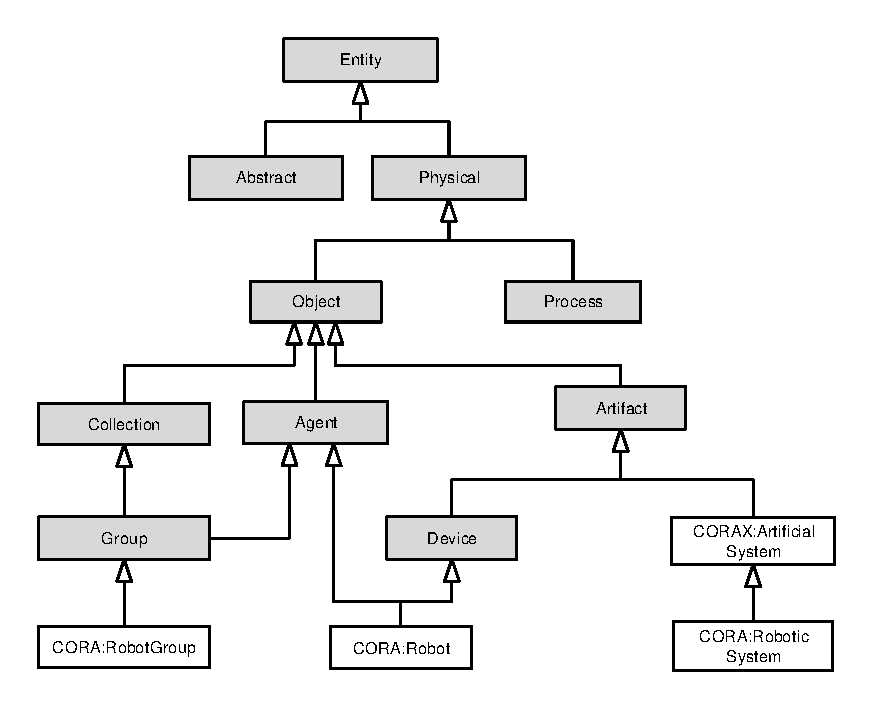
\includegraphics[width=1\textwidth]{figs/cora}  
	\caption{Overview of the main concepts in CORA: \emph{robot}, \emph{robot group} and \emph{robotic system}}  
	\label{fig:completeontology}  
\end{figure}  


The term \textit{robot} may have as many definitions as there are people writing about the subject. This inherent ambiguity in the term might be an issue when specifying an ontology for a broad community. We, however, this ambiguity as an intrinsic feature of the domain, and therefore have decided to use a definition based purely on necessary conditions, without specifying sufficient conditions. Thus, our goal is to ensure that CORA's definition of robot includes most of the entities that the community actually considers as robots, at the cost of classifying as robots some entities that actually are not considered as robots in the point of view of some roboticists. However, the concepts in our ontology could be extended according to the needs of specific sub-domains or applications of R\&A.

More importantly, our definition of robot emphasizes its functional aspects. For our general purposes, {\it robots are agentive devices} in a broad sense, designed to perform purposeful actions in order to accomplish a task. In some cases, the actions of a robot might be subordinated to actions of other agents, such as software agents (bots) or humans. Robots are also \emph{devices}, composed of suitable mechanical and electronic parts. Robots can form \emph{social groups}, where they interact to achieve a common goal. A robot (or a group of robots) can be combined with other devices to form robotic systems. An environment equipped with a robotic system is a robotic environment.

%TODO Esta frase não é mais verdadeira
%A robot (or a group of robots) can form robotic systems together with specially prepared environments. 

A {\it robot} is a {\it device} in the sense of SUMO. According to SUMO, a device is an artifact (i.e., a {\it physical object product of making}), which participates as a tool in a process. Being a device, robot inherits from SUMO the notion that devices have parts. Therefore, CORA allows one to represent complex robots with robot parts.

%A {\it robot} is a {\it device} in the sense of SUMO. According to SUMO, a device is an artefact (e.g. a{\it physical object product of making}), {\it which participates as a tool in a process}. Naturally, a device can have parts. We define an specific concept called {\it Robot Part}\footnote{In summary, Robot Part is what is called {\it Formal Role} in \cite{GUARINO:2000} or {\it Role Mixin} in \cite{GUIZZARDI:2005}, that is, an anti-rigid and externally dependent class that abstracts many roles of classes with different identity criteria. For example, considering the class {\it Actuator}, we could have a class {\it Actuator As Robot Part} that dynamically classify actuators when they are connected to Robots. Thus, {\it Robot Part} generalizes {\it Actuator As Robot Part} and some other {\it roles} such as {\it Gripper As Robot Part} }, which can classify any other device that can compose a robot, from nuts and bolts to manipulators and actuators. 

A robot is also an {\it agent}. SUMO states that agent is ``{\it something or someone that can act on its own and produce changes in the world}''. Robots perform tasks by acting on the environment or themselves. Action is strongly related to agency, in the sense that the acting defines the agent. A robot can form robot groups. A \emph{robot group} is also an agent in the sense that its own agency emerges from its participants. This notion can be used to describe robot teams, or even complex robots formed by many independent robotic agents acting in unison.

%TODO JOEL: Este parágrafo não corresponde mais à nossa modelagem atual.
%Robots can ultimately participate in {\it robotic systems}. Certain environments are prepared in such a way that they facilitate the operations of robots. These environments, together with the actual robots are called robotic systems. A good example of a robotic system is a car assembly cell in a car factory. It is formed by an environment prepared with actuated structures that manipulate the car frame, so industrial robots can act on them. 

{\it Robotic systems} are systems composed of robots (or robot groups) and other devices that facilitate the operations of robots. A good example of a robotic system is a car assembly cell at a manufacturing site. The environment is equipped with actuated structures that manipulate the car body in a way that the industrial robots within the system can act on it. Finally, as previously stated, an environment equipped with a robotic system is a {\it robotic environment}.
See \cite{prestes2013towards,carbonera2013defining} for a more detailed discussion on CORA's main concepts. Next, we describe new notions that have been integrated into CORA. 


\section{Updating CORA}

CORA has been updated since its initial proposal in \cite{prestes2013towards,carbonera2013defining}. The main driving force behind these changes came from aligning it with existing ontologies and more expert involvement in the development process. We compared CORA with an application \textit{ontology for kitting} developed within the group \cite{balakirsky2013knowledge}.This enabled us to investigate whether or not both ontologies could be merged, and to check whether all notions in the kitting ontology were represented in the combination of SUMO and CORA. We found that important concepts and relations present in the kitting ontology that were not covered. Due to this, we developed new ontology modules to bridge the gap between SUMO and the kitting ontology, which are mostly covered by CORAX and the POS ontologies.

Furthermore, after the preliminary draft standard was completed, we experienced increased involvement of independent experts and received additional feedback. Apparently, experts were more comfortable discussing concepts and relations, after a first set of ontological commitments were made and the scope of the project was established. The initial model served as a reference to articulate new requirements on the ontology. Since the initial model was based on well-founded ontological commitments, the model was more resilient to ad-hoc proposals to change it, translating into a more stable evolution of the ontology. Notably, changes were more prominent in aspects of the ontology that had a less solid foundation in the first version of the ontology, such as autonomy. 
%Very good!

In the following sections, we describe the changes made in and around CORA as a result of that process. They consist mostly of sub-ontologies complementing or extending CORA (see Fig.~\ref{fig:modules}).

\begin{figure}[th] 
	\centering  
	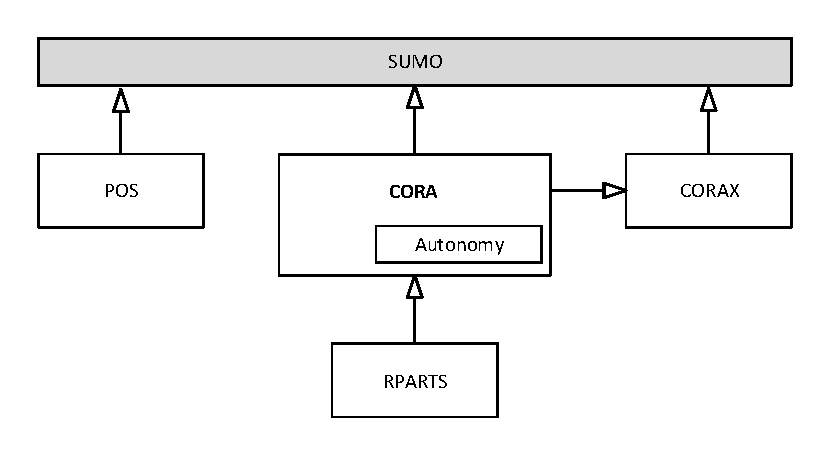
\includegraphics[]{figs/modules}  
	\caption{Extensions made to CORA and SUMO. CORAX, POS and RPARTS are extensions made to SUMO and CORA. The way CORA represents autonomy was also updated.}  
	\label{fig:modules}  
\end{figure} 

%\joel{I think we need to explain more what the boxes are representing.}
%\Sandro{Note to myself: change the figure. Fill SUMO box like CORA.}

\section{CORAX: connecting CORA and SUMO}

Naturally, SUMO does not cover every possible aspect of reality, even when we restrict ourselves to R\&A. At the same time, some of parts of reality are too general to be included in CORA. We introduced the CORAX ontology to address this problem by bridging SUMO and CORA. In particular, CORAX includes concepts and relations associated with design, interaction, and environment that are not covered in SUMO.

\subsection{Design}

Design is an important concept in engineering, specially in manufacturing. In R\&A, the concept is frequently related to industrial robotics, where robots perform the job of building artifacts. Those robots have to know the design of the artifacts they are building in order to coordinate their actions. 

A design is an abstract entity; it does not have materiality in itself. Rather, \emph{content-bearing objects} (in SUMO), such as manuals and blueprints, give materiality to a design. One could reason this in another way: a design is what links a series of related \emph{blueprints}; it is the common abstract content that is represented in different blueprints. Furthermore, an artifact is related to a particular design, so that one should expect that the \emph{artifact} realizes the design.

%\Sandro{we might have to relate this with the literature in design ontologies}


From our point of view, SUMO does not provide a good specification of design. One of its sub-ontologies---namely the engineering ontology---defines the concept \emph{Model}, which is an abstract entity that seems to capture the notion of design described above. However, a model is not clearly related to content bearing objects, or to \emph{artifacts} in general. SUMO defines a relationship called \emph{models}, which is held between \emph{Model} and \emph{Engineering Component}. However, this relationship is too restrictive for our purposes, since we would like to represent models of any kind of artifact. 

In response to this, we defined the concept of \emph{Design}, which is a kind of \emph{Proposition}. According to SUMO, a \emph{proposition} is an abstract entity that expresses a complete thought or a set of thoughts. For instance, the phrases ``\textit{the cat is on the mat}'' and ``\textit{o gato est\'{a} no tapete}'' express the \emph{same} \emph{proposition} in English and in Portuguese, respectively. In much the same way, different \emph{blueprints} might express the same \emph{design}. 


\begin{figure}[th]
    \centering
    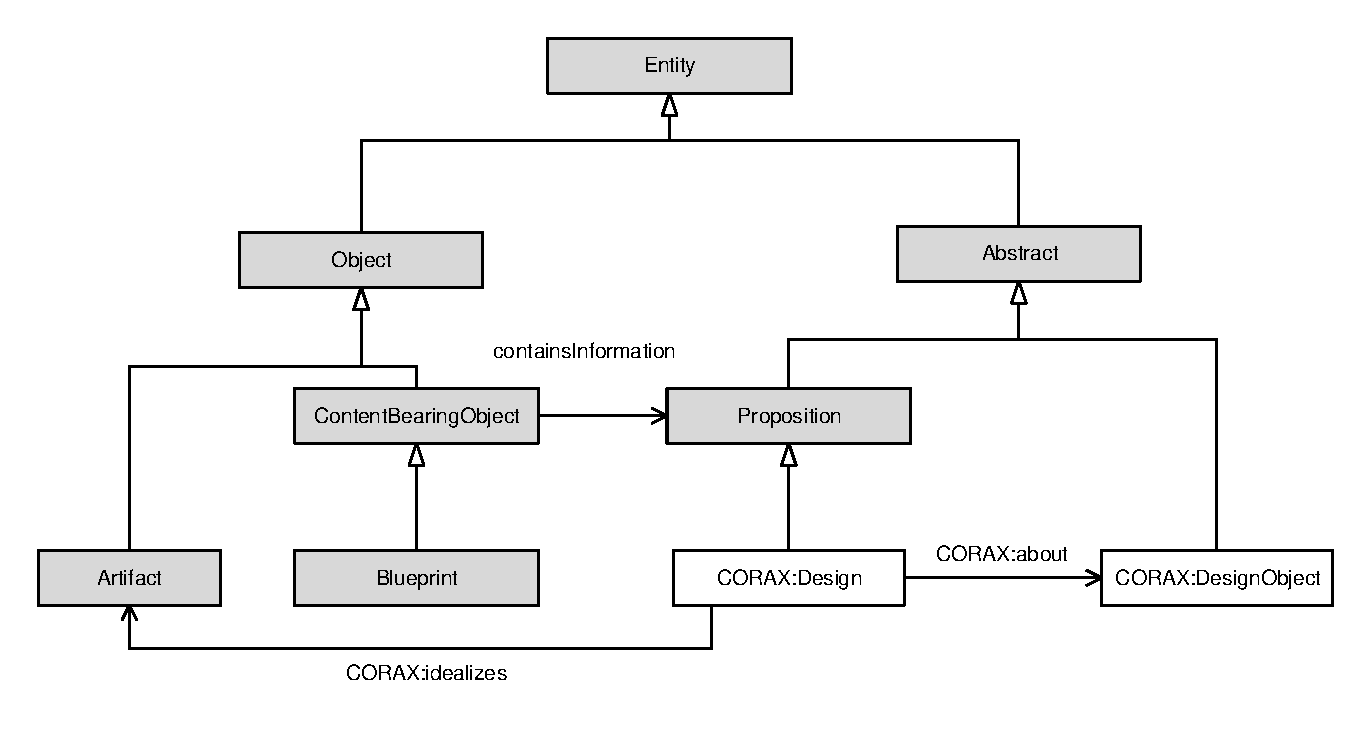
\includegraphics[width=1\textwidth]{figs/design}
    \caption{Entities associated with Design in CORAX.}
    \label{fig:design}
\end{figure}


Furthermore, the properties of the object must be expressed in its design. For instance, the design of a phone is about an ideal (\emph{idealized}) phone that is materialized in the individual realizations of the design. This ideal phone has ideal properties, such as ideal weight and shape. There are many ways of representing an idealized object within an ontology. For instance, one could represent it as a special instance of the concept \emph{Phone}, called prototype. Another alternative is to collapse both the design and the ideal object into the same entity. This is exactly the approach that was adopted in the design ontology that is presented in \cite{Storga2010design}, which is also based on SUMO. However, since the ideal object is also a proposition, there might be issues when modelling its attributes and parts. For instance, if both the design of a phone and the ideal phone (the content of the design) are the same entity, this entity, as a proposition, will have a designed color and a designed shape. However, \emph{a proposition cannot have a color or a shape}. Thus, we model the ideal object as a separate abstract entity called \emph{Design Object}, which specifies the idealized object that is the \emph{content} of a Design. We believe this definition better matches the experts' intuitive notion of an engineering model; it also eliminates the need for a new metacategory in SUMO (such as prototype). As with physical objects, design objects have properties such as weight and shape. SUMO provides two main relations to represent properties, namely \emph{attribute} and \emph{measure}, but these can only predicate physical objects. We therefore created the relations \emph{designAttribute} and \emph{designMeasure}, which are analog to attribute and measure in SUMO, reusing their domain values. In this way, we can specify that, for instance, an idealized phone (an instance of \emph{Object Design}) has a \emph{design shape} and a \emph{design weight}. 

%A complex design ontology based on SUMO was presented in \cite{Storga2010design} that collapses both entities as one. 

%\joel{In my point of view, talking about the metacategory prototype will make this paragraph a little unclear. If we decide to talk about this, we need to provide more details and justifications.}
%\paulo{no need, in my opinion.}

Designs \emph{idealize} artifacts (therefore, the relation \emph{CORAX:idealizes} in Figure \ref{fig:design}). It is important to note that it is the \emph{design} that idealizes the artifact, and not the design object. The properties of the design object and those of the artifact may correlate, but we will not provide a theory about how this correlation occurs at this stage.
%\joel{Vitor has said that in his point of view the relations between properties in the artifact and properties of the design object are less mysterious than our text express. In general, the correlation occurs because the properties of the design object are ideal goals that are pursued during the manufacturing process. The process of manufacturing succeeds only when a high correlation is achieved between the properties of the design object and the artifact.}
%\Sandro{This is an excelent point, but we do not have time to further explore that issue.}
%\joel{Actually, Vitor has pointed out that in the way that it is, our text overcomplexify a point that does not have to be so complex. That is, the correlation exists I have provided that explanation about the correlations as a try.}

\subsection{Physical Environment}

Another important notion missing in SUMO is that of \emph{physical environment}. We added this concept to CORAX in order to support specification of \emph{robotic environments}. In our view, an \emph{environment} is intuitively composed of a physical region, plus other eventual physical entities that characterize the environment. In addition, the definition of physical environment depends on the presence of a landmark (another physical entity) from which it is possible to define the main region of an environment. Landmarks may or may not be located within the region of interest of the environment. For instance, an office room environment depends on the physical configuration of its walls, which are located in the environment. But we can also define an arbitrary environment consisting of a cube in outer space that depends on Earth as a landmark. In this case, Earth does not need to be located within or at the borders of the region.


\begin{figure}[h]
    \centering
    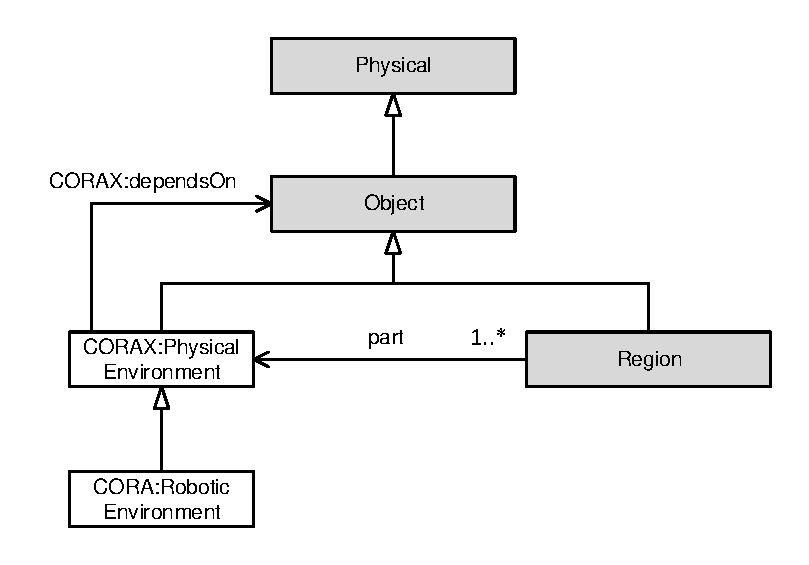
\includegraphics[width=0.7\textwidth]{figs/physicalenv}
    \caption{Concepts and relations of Physical Environment in CORAX.}
\end{figure}

More formally, we define a physical environment in CORAX as a physical object that has at least one region as \textit{part} and that depends on another entity. All other physical objects that are part of an environment must be located within a region that is part of the environment.
%\paulo{clear enough, but can we have a mathematical definition here, or have decided not to include it in the text.}

\subsection{Interaction and Artificial Systems}

In order to properly define a \emph{robotic system}, we have to specify what is an \emph{artificial system}. An artificial system is simply an artifact formed from various devices and other objects that interact with each other and with the environment in order to fulfill a function. 

This requires a basic definition of \emph{interaction}. We define interaction as a process in which two agents participate, where an \textit{action} generated by one agent causes a \textit{reaction} by the other. More specifically, an interaction process is composed by two sub-processes corresponding to action and reaction. The action sub-process initiated by $x$ on $y$ causes a reaction sub-process, where $y$ acts upon $x$.


\section{CORA: Autonomy revisited}


\textit{Autonomy} is one of the most important terms in R\&A, yet one of the hardest to  define precisely. In the previous version of CORA, we advocated for a flexible definition that --- while not being precise --- could distinguish between robots that were clearly autonomous from others with questionable autonomy. In CORA, it has now been pushed a step further in order to make the modelling more versatile. 

In this new version, our definitions are aligned with those from the ALFUS \cite{huang2003toward} framework, which was the result of an extensive study on autonomy in unmanned vehicles. In short, ALFUS states that autonomy is generally dependent on the \textit{degree of human intervention} and \textit{context}, where the latter is characterized by \textit{type of mission} and \textit{environment}. 

CORA's definition of autonomy is closely related to what ALFUS defines \emph{modes of operation for unmanned systems}. These modes stretch from fully autonomous to remote controlled, representing the degree of human interaction needed for the robot to perform its task. In our view, they encapsulate the experts' intuitive notion of autonomy in R\&A\footnote{ALFUS goes a step further in trying to characterize absolute levels of autonomy, which  correlates with the modes of operation presented here. However, the exact nature of this relation is not clarified.}. More specifically, CORA includes:

\begin{description}
    \item[\emph{Fully autonomous robots}:] A role for a robot performing a given task, in which the robot solves the task without human intervention, while adapting to operational and environmental conditions. 
    \item[\emph{Semi-autonomous robot}:] A role for a robot performing a given task, in which the robot and a human operator jointly plan and conduct the task, requiring various levels of human interaction. 
    
    \item[\emph{Teleoperated robot}:] A role for a robot performing a given task, in which a human operator either directly controls the actuators using sensory feedback, or assigns incremental goals on a continuous basis. A teleoperated robot will complete its last command after the operator stops sending commands, even if that command is complex and time-consuming. 
    
    \item[\emph{Remote controlled robot}:] A role for a robot performing a given task, in which the human operator controls the robot on a continuous basis, from a location off the robot via only her/his direct observation. In this mode, the robot takes no initiative, and relies on continuous, or nearly continuous input from the human operator.
    
    \item[\emph{Automated robot}:] A role for a robot performing a given task, in which the robot acts as an automaton, following pre-defined (scripted) plans, not adapting to changes in the environment.
\end{description}

It is important to note that \emph{automated robot} is not part of ALFUS' modes of operation. Experts in our groups determined that certain robots require little human interaction, but at the same time are too simple to be characterized as autonomous. This is the case of automatons, including automated dolls and toys, which \emph{cannot} react to changes in environment. Relatively simple code scripts or mechatronics determine the behavior of these robots.  

%\joel{The paragraph bellow is a kind of weird. I'm not sure if I understood it correctly.}

One could mention at this point that some robots are inherently autonomous, or at least, are made with this purpose in mind. Therefore, autonomy would not depend on context. Indeed, there is a correlation between purpose and physical capabilities of a robot, and the modes of operation it can achieve in certain tasks. Yet, this is not the definitive factor in how the robot will operate during its lifetime. It only means that such a robot \emph{can} play a role of autonomous robots.

The fact that this classification of autonomy is context-dependent also affected our modelling choices. In a modelling sense, a mode of operation is a \emph{role}. A role can predicate a given entity at a given time, but it can cease to predicate it at a later time. For instance, the canonical example of role is \emph{Student}: one can predicate a person as a student at a given time, and later cease to do so. This contrasts with rigid types, such as \emph{Person}. Someone cannot cease to be a person without ceasing to exist. That is, someone cannot cease to be a person without ceasing to exist. In general, a role is also dependent on another entity. For instance, a person must be enrolled at an educational institution in order to be predicated as a student.

A modeler can specify roles in many ways. The earlier version of CORA specified the various modes of operation as concepts. However, SUMO does not support roles as concepts (contrary to other ontologies \cite{Guizzardi2005}). For that reason, we modified the modelling of operational modes so that they became a specific type of relation present in SUMO, namely \emph{Case Role}.

A case role in SUMO is a \emph{relation} between an entity and a process. It describes a role that an entity plays in the process in which it participates. In order to define autonomy levels as case roles, we specialized the relation \emph{agent} present in SUMO into the relation \emph{robotAgent}. The relation agent links entities to the processes where they have an ``active determinant'' behavior. The relation \emph{robotAgent} applies to robots and the processes in which the robot is the active determinant. A given operational mode depends on the way a robot determines the outcome of the processes it is involved in. We represent the operational modes as a subrelation of robotAgent: \emph{fullyAutonomousRobot}, \emph{semiAutonomousRobot}, \emph{teleoperatedRobot}, \emph{remoteControlledRobot} and \emph{automatedRobot}. When a particular robot assumes a particular operational mode for a particular task, it is predicated with the appropriate relation. For instance, a robot that can drive autonomously, assumes the role \emph{fullyAutonomousRobot} for the autonomous driving process. The same robot can assume different operational modes in different processes, depending on the context. Interestingly, since processes can have sub-processes, a robot can assume different roles for different sub-processes. For instance, a cleaning robot might be fully autonomous as it detects dirty places to clean, but simultaneously be semi-autonomous with respect to planning routes around the house, or vice versa. %For instance, a cleaning robot might be fully autonomous regarding planning routes around the house, but semi-autonomous at detecting dirty places to clean. 

%\Sandro{People might criticize why robot interface and interaction is not related to autonomy, given the later one is built on degrees of human interaction}


\section{RPARTS: Robot parts and extensibility}

%\Sandro{Main point: also modelling as roles.} 

%There exists a multitude of devices and parts that compose robots.

%- No part is necessarily part of a robot. For instance, ... (a laser? a sonar?)

%- A device is a robot part only when it is attached to a robot.

%- No contextual dependencies. Initial modelling as concept.

%- Limitations of this modeling choice in the context of SUMO. Modality in SUMO. Limitations of case roles.

%- Change to relation. Relations have a role flavor.

%- There is a need for an ontology of parts. Modularity. Nedd for specific ontologies of devices that can play the role of robot part.
RPARTS is a sub-ontology of CORA that specifies the notions related to specific kinds of robot parts.

According to CORA, robots are (agentive) devices \emph{composed of} other devices. A myriad of devices can be robot parts, and we cannot determine in advance what \emph{kinds} of devices can or cannot be robot parts. Notice that this is an issue that arises at the \emph{conceptual level}. This is a consequence of the ``open-ended'' nature of robots, whose designs are only constrained by human needs, human creativity and available technological resources. Therefore, a type of device that has never been considered as a potential robot part can be used as a robot part by some future designer. An ontology for R\&A, as CORA is, must take this issue into account.

Furthermore, there is another issue regarding the notion of robot parts that arises at the \emph{instance level}. According to our analysis, none of the instances that can be classified as robot parts are \emph{essentially} robot parts, since they can exist by themselves when they are not connected to a robot (or when they are connected to other complex devices). For instance, a power source is essentially a device, and we cannot consider power source as a sub-class of the class of robot parts, because this would imply that all instances of power sources are always robot parts. This is not true, since a specific instance of power source can be dynamically considered as a part of different complex devices during different specific time intervals. Due to this, CORA assumes that the notion of ``robot part'' is a \emph{role} (in the sense previously discussed) that can be played by other devices.  %A \emph{role} can be broadly understood as a class that some instances can assume dynamically in specific contexts such as a specific person becoming a student, a specific device becoming part of a robot.

%The matter of robot parts can be seen as a domain on itself. Thus, we consider that it is not suitable for inclusion in the core ontology. However, the core ontology must provide a way for classifying devices as robot parts as needed. Due to this, we decided to abstract the notion of robotic part as a role. 


In the earlier version of CORA \cite{prestes2013towards}, the notion of robot part was considered as a \emph{class}, whose instances are not \emph{essentially} instances of it. Thus, instances of robot part could cease to be robot parts, without ceasing to exist. In this sense, for example, an instance of power source that is considered as a robot part at a given moment (when it is connected to a robot) could cease to be a robot part in another moment without ceasing to exist (as an instance of power source). Thus, \textit{Robot part} was considered as an \emph{anti-rigid} class, in the sense of \cite{Guarino2009,Guizzardi2005}. Our modelling pattern \cite{prestes2013towards} was developed accordingly, inspired by \cite{Guizzardi2005}. It represents how a specific instance of a specific kind of device (e.g., power source) could be classified as a robot part.

This pattern becomes complex when we take into account the principles advocated in \cite{Guarino2009,Guizzardi2005}. According to these frameworks, an anti-rigid class (e.g., robot part) cannot subsume a rigid one (e.g., power source). Considering this principle, for each rigid class $c$ that can play the role of robot part, we must create another specific anti-rigid class (a specific role) that will be subsumed by both $c$ and \emph{Robot Part}. For example, an instance of the rigid class \emph{Wheel} only becomes a robot part when it is attached to a particular robot. Given this condition, it becomes a member of the more specific class (e.g., ``\emph{Wheel as Robot Part}''), which is subsumed by the rigid class \emph{Wheel} and the anti-rigid class \emph{Robot Part} (see \cite{prestes2013towards} for further details.)

The representation of robot parts in the new edition of CORA was changed, mainly because the modelling pattern proposed for representing robot parts results in domain models that are overwhelmingly complex. Some classes that must be created in order to maintain the consistency of the model do not fit well into the domain conceptualization, and the resulting complexity is hard to manage. Therefore, this modelling pattern could hinder the broad adoption of the ontology in the domain. Another factor leading to the revision was that it is not clear how to fit the dynamical behavior that is expected from roles in the framework of SUMO. The modelling of roles adopted in \cite{Guarino2009,Guizzardi2005} relies on the notion of \emph{possibility} (a \emph{modal} notion). However, as pointed out in \cite{oberle2007dolce}, the treatment of possibilities in SUMO is not clear.

%In order to understand our current modelling of robot part, it is necessary to understand how SUMO treat the roles. In general, the literature distinguishes two main types of roles: \emph{processual roles} and \emph{relational roles}. 

%Processual roles are played by entities when they participate in some process; corresponds to the manner in which a single participant behaves in some process. For example, when a robot moves a box, the robot plays the role of agent, while the box play the role o patient. SUMO allows the modelling or processual roles through the notion of \emph{case roles}. However, the notion of robot part does not seem to be suitably captured as a processual roles. A device does not play the role of robot part by virtue of participating in a process.

%Relational roles, on the other hand, are played by entities in some contexts, when they are related to other entities; that is, they correspond to the way in which an entity participates in the context of some relationship. For examples, student is a role played by a person when she is enrolled at an educational institution. SUMO provides an approach for modeling a notion that is similar to relational role through the the so called \emph{relational attributes}, which, according to SUMO, is \emph{any attribute that an entity has by virtue of a relationship that it bears to another entity or set of Entities}. Notice that in this modelling strategy a role is not class that can dynamically classify different individuals in different contexts. Rather, it behaves as an attribute. Also, it is important to notice that using relational attributes, sub-roles needs to be modelled using the notion of sub-attribute. We have decided to use relational attributes for modelling the notion of robot part.

In the current version of CORA, we have modeled the notion of robot part as a relationship between a given device $d$ and a robot $r$, indicating that $d$ is playing the role of robot part when it is connected to $r$. During the analysis of the domain literature, we identified some specific types of parts that are important to distinguish within the notion of robot part. These types of parts --- according to our analysis --- would be different sub-roles of robot part, which could be played by devices with specific features. Thus, robot parts in CORA can be:

\begin{description}
    \item[\emph{Robot sensing part}:] responsible for sensing the surrounding environment. Formally, robot sensing parts must be measuring devices connected to the robot. A measuring device, according to SUMO, is \emph{any device whose purpose is to measure a physical quantity}. For example, a \emph{laser sensor} can play the role of robot sensing part, when connected to a robot.
    \item[\emph{Robot actuating part}:] responsible for allowing the robot to move and act in the surrounding environment. Formally, robot actuating parts must be devices that are instruments in a process of robot motion, which is any process of movement where the robot is the agent and one of its parts is acted upon.
    \item[\emph{Robot communicating part}:] responsible for providing communication among robots and humans, by allowing the robot to send (or receive) information to (or from) a robot or a human.
    \item[\emph{Robot processing part}:] responsible for processing data and information. Formally, robot processing parts must be processing devices connected to the robot. A processing device is any electric device whose purpose is to serve as an instrument in a subclass of computer process.
\end{description}

It is important to emphasize that although these different types of robot parts are modeled as relations between specific devices and robots, they are intended to behave as roles. 

This modelling choice also provides interesting modularity characteristics. It keeps CORA as a minimal core of high-level concepts that provide the structure to the domain without going deep into details regarding the myriad of different devices that could play the roles specified here. In this sense, this structure of roles can be viewed as an interface (in the sense of \emph{object oriented programming paradigm}) that can be implemented in different ways. Naturally, this schema the need for sub-ontologies to define the taxonomies of devices that can play the roles specified in CORA, such as an \textit{ontology of sensors, ontology of grippers}, etc.   
 

%\section{Robot interaction}


%\joel{I'm not sure about the section about interaction. It seems that we don't have content enough about interaction for a section.}
%\paulo{ok to delete.}



\section{POS: Position, orientation and pose}

The position (POS) ontology is an ontology that extends SUMO and complements CORA. POS was developed for capturing the main concepts and relations underlying the notions of \emph{position}, \emph{orientation} and \emph{pose}. These  are essential for dealing with information about the relation between the robot and its surrounding space. In this section, we summarize the main concepts relating to positional information. Figure \ref{fig:POS} presents an overview of some of the main notions captured in POS, showing their relationships with concepts of SUMO.

\begin{figure}[h]
    \centering
    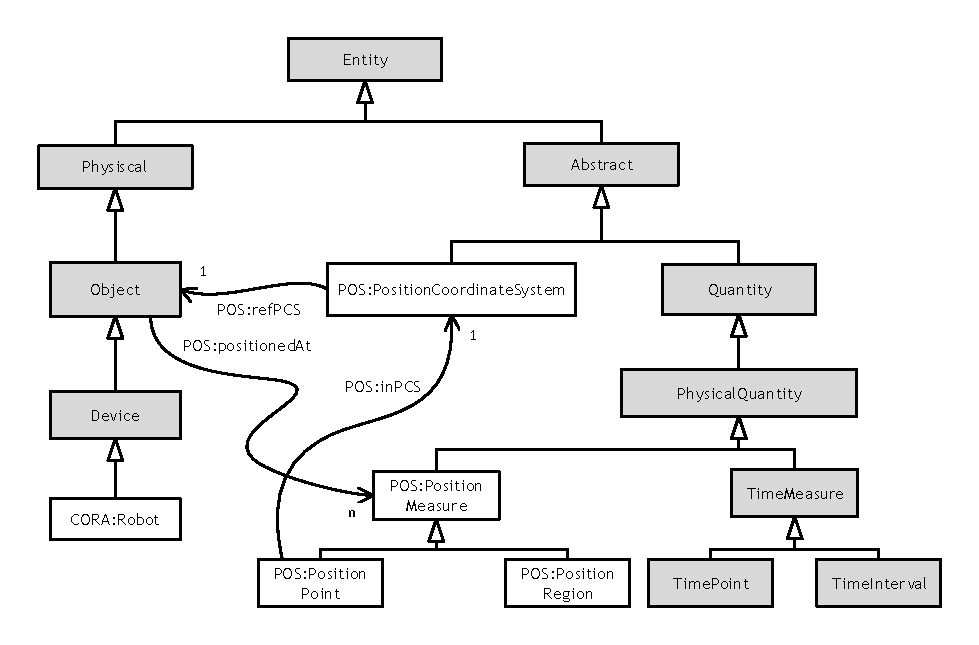
\includegraphics[width=1.0\textwidth]{figs/pos}
    \caption{Fragment of POS ontology, presenting the main concepts and relations underlying the notion of \emph{position}.}
    \label{fig:POS}
\end{figure}

According to the literature, roboticists and other domain experts usually utilize two kinds of positional information \cite{ye2007unified}: \emph{quantitative} and \emph{qualitative}. In the quantitative case, a position is represented by a \emph{point} in a given coordinate system. In the qualitative case, a position is represented as a \emph{region} defined as a function of a reference object. For instance, one can describe a robot as being positioned at the coordinates $(x, y)$ in the global coordinate system, or that the robot is positioned \emph{at the front of the box}, where \qm{front} comprises a conical region centered on the box and pointed forward.

%\joel{Interesting...According to our example, it seems that the region has a orientation (pointed forward)}
%\paulo{normally a region must have a center a normal, pointing to outside that region}

We consider that a \emph{position} can be attributed to a (physical) \emph{object}. In this sense, when we say that ``a robot x is positioned at y'', this means that there is a \emph{measure} that relates a given ``robot x'' to a \emph{position measurement} \emph{y}. 

\emph{Position measurements} are \emph{physical quantities} that can be \emph{position points} or \emph{position regions}. A position point refers to a point in a \emph{coordinate system} projected on the physical space. A position region is an \emph{abstract region} in a \emph{coordinate system} defined with reference to a series of position points.

A position point denotes the \emph{quantitative} position of an object in a coordinate system. More specifically, position points are always defined in a single coordinate system.

A \emph{coordinate system} is an \emph{abstract} entity that is defined in relation to \emph{a single reference} object, i.e., there is an object that is the reference for each coordinate system. For instance, the local coordinate system of a robot is referenced by the robot itself. Additionally, the reference object does not need to be at the origin of the coordinate system.

This ontology does not commit to a particular kind of coordinate system. It can be stated however, that a coordinate system defines at least one dimension in which points get their coordinate values. An $n$-dimensional coordinate system, $c$, is homeomorphic to a subset of $\mathbb{R}^n$, such that a coordinate $p \in c$ can represented as  $n$-tuple $\phi(p) = (x_1(p), x_2(p), \dots , x_n(p))$. The functions $x_1, x_2, \dots, x_n$ are coordinate functions that attribute to $p$ a real value in the dimension $n$ of the coordinate system \cite{Morita2001Geometry}.

A fundamental aspect of coordinate systems is the notion of \emph{transformation}, which maps position points in one coordinate system to position points in another coordinate system. Transformations can be composed generating new transformations. In our ontology, an object can display multiple positions in different coordinate systems only if there is a transformation that can map between the two.

In addition, coordinate systems are related through \emph{hierarchies} (i.e. trees). We say that a given coordinate system $c_\mathit{1}$ is parent of a coordinate system $c_\mathit{2}$ if there is a transformation $t_\mathit{1}$ that maps the points of $c_\mathit{1}$ to points in $c_\mathit{2}$, and there is a transformation $t_\mathit{2}$ that maps the points of $c_\mathit{2}$ to points in $c_\mathit{1}$. According to this, if two coordinate systems share a parent node in the hierarchy tree, there is a transformation between them. Usually, an agent chooses a coordinate system as the global reference frame that constitutes the \emph{global coordinate system} (GCS) for that agent. This GCS can be \emph{arbitrarily} chosen and does not have reference to a particular coordinate frame. \emph{Local coordinate systems} (LCS) are defined in relation to GCS by hierarchical links. This hierarchy is arbitrary, in the sense that it can be defined by the designer or agent.

As already stated earlier, besides the quantitative position, our ontology also provides concepts about qualitative positions that are defined in terms of position regions. Example of qualitative positions are ``left of'', ``in front of'', ``on top of'', etc. These expressions define regions in relation to a reference object $o_r$ in which other objects are placed. More specifically, a \emph{position region} is composed of poses in the coordinate system generated by a \emph{spatial operator} on the reference object. The spatial operator is a \emph{mathematical function} that maps reference objects to regions in a coordinate system in arbitrary ways.

Our ontology also allows for the representation of \emph{relative positions} of objects with respect to a given reference object. In general, this kind of information is represented through \emph{spatial relations} that hold between objects. An example of this kind of information is the relation $\mathrm{leftOf}(o, o_\mathit{r})$, which represents that the object $o$ is positioned to the left of the object $o_\mathit{r}$. This kind of relation can be defined in our framework using the notions of \emph{relative position} and \emph{spatial operator}. For example, the relation $\mathrm{leftOf}(o, o_\mathit{r})$ holds when there is a qualitative position $s$ (a position region) that was generated by the spatial operator $\mathrm{leftOfOp}$ over the reference object $o_\mathit{r}$, and the object $o$ has the relative position $s$ regarding $o_\mathit{r}$. Through this mechanism, our ontology provides the semantics for spatial relations like \qm{to the left of}.

The usual notion of orientation is similar to position as far as its conceptual structure is concerned. Due to this, we will provide only a brief overview. An object can have a quantitative orientation defined as a value in an orientation coordinate system, as well as a qualitative orientation defined as a region in relation to a reference object. For example, orientation is used in the phrase \qm{the robot is oriented at 54 degrees}; the orientation value in this case is 54 in the circular, one-dimensional coordinate system of a compass. On the other hand, orientation regions capture a less intuitive notion. The expression \qm{the robot is oriented to the north of the Earth} allows for interpretations where the robot has a range of possible orientation points around 0 degrees. Thus, we model \qm{north} as a region (or interval) in the one-dimensional compass coordinate system that overlaps with the general orientational extension of the object.

A position and an orientation constitute a pose. The pose of an object is the description of any position and orientation simultaneously applied to the same object. Often, a pose is defined with a position and an orientation referenced to different coordinate systems/reference objects. In addition, since objects can have many different positions and orientation, they can also have many different poses.

It is important to note that the current version of the POS ontology is \emph{synchronic}. That is, it considers only facts about a single time point, just like a snapshot in time. One of the future extensions to this ontology will consider dynamic world modelling, eventually producing a \emph{diachronic} version of the POS ontology.


\section{Discussion}

The importance of information sharing in R\&A emphasizes the necessity of standardization in the field. These standards must be \emph{clear}, \emph{precise} and \emph{easy to use}. CORA is designed to meet that need: it specifies the central concepts of R\&A and related fields. In this paper, we presented new additions to CORA and its adjoint domains, providing concepts about positioning, autonomy (including modes of operation), and interaction. These can already be used for building more detailed sub-domain ontologies and algorithms. 

Several scenarios could take advantage of CORA (and the related ontologies) in R\&A. Firstly, CORA can be immediately applied in offline \emph{meaning negotiation} among roboticists. That is, our ontologies could be used as \emph{reference conceptual models} for ensuring mutual agreement among humans regarding the meaning of concepts of R\&A domains. 

Moreover, used as a \emph{software component}, the ontology can naturally be applied for enhancing communication among (heterogeneous) robots, as well as among robots and humans. For example, a straightforward application for CORA is as a tool developing a \emph{middleware} for communication, ensuring semantic interoperability between the members of a robot group.

Our ontologies can be used as \emph{reusable knowledge components} in \emph{knowledge-based problem-solving processes}. Using CORA, thus, a robot can apply high-level logical reasoning capabilities, taking advantage of its high-level knowledge about the world to decide which action it should perform in order to achieve its goal. In general, robots can use ontologies to support tasks such as \emph{planning} \cite{provine2004ontology,galindo2008robot,belouaer2010ontology} and \emph{navigation} \cite{bateman2005modelling}. Other ontologies can also be integrated with our ontologies, providing a wide range of concepts and relations that allow richer descriptions of the robot's world. Such semantic descriptions can be used by the robot in perception processes such as \cite{modayil2007autonomous,suh2007ontology,johnston2008ontology,lim2011ontology} for enhancing tasks that require \emph{object recognition} through \emph{visual perception}. These semantic descriptions can be used for specify tasks to the robot, as in \cite{stenmark2013knowledge}.

%And, as proposed in approaches such as \cite{modayil2007autonomous,suh2007ontology,johnston2008ontology,lim2011ontology}, these semantic descriptions can be used by the robot in tasks that require object recognition through visual perception, for example.   

%Our ontologies can also integrate other ontologies that describe the ordinary objects of the robot's environment. With such a broad ontology, it is possible to provide a richer description of the robot's world. As proposed in approaches such as \cite{modayil2007autonomous,suh2007ontology,johnston2008ontology,lim2011ontology}, ontologically well-founded descriptions can be used by the robot in tasks that require object recognition through visual perception, for example.   

Furthermore, our ontologies can be used for defining the notions underlying \emph{robot programming frameworks}. CORA could provide these frameworks with a conceptual structure that fits the conceptualization that is shared among the roboticists. For instance, an object-oriented programming framework for robots based on concepts and relations in CORA would be more easily assimilated by new programmers. In this way, dealing with these frameworks would become more natural for the practitioners of R\&A. In addition, our ontologies could define standard \emph{interfaces} for these frameworks, promoting the semantic interoperability among them. %In this way, the adoption of CORA in such frameworks could increase the \emph{productivity} in the field. 

CORA can also be used for promoting \emph{data integration} and \emph{semantic interoperability} among robot databases. This could have positive impacts to the \emph{knowledge management} process of companies that commercialize products and components for the R\&A field.

%How cora can be used by the community:
%-Communication: robot-robot, human-robot
%-Problem-solving: reasoning, planning, visual recognition
%-Robot programming
%-knowledge management and data integration for companies that develop robots.

\section{Future work: what should we expect next?}

CORA and related ontologies still do not cover some important areas in R\&A. For instance, \emph{control} still needs to be taken into account. This issue is complex, since it involves other important concepts in robotics, such as perception, planning, and action. CORA should also incorporate information ranging from simple classical controllers --- such as proportional-integral-derivative controllers (PID) --- to complex non-linear control. In addition, it should also account for different control strategies. 

%that by the way need to also developed. only found this one An Ontology-Based Expert System and Interactive Tool for Computer-Aided Control Engineering Education}

The notion of \emph{task} is also important in this domain. Since robots should be able to operate in complex scenarios, task definitions must be clear to allow robots to communicate with each other, other machines, and humans. In this sense, ontologies play a clear role in task specification. CORA must be designed to allow several types of tasks in various environments, e.g., grasp, move, scan, and so on. Future work will be devoted to the ontological characterization of what kind of entity a task is. For example, we believe that a good starting point is to separate \emph{tasks} from \emph{task executions}. With this distinction, we acknowledge that tasks are \emph{abstract} entities that describe goals to be reached; while tasks executions are \emph{events} composed by \emph{actions} that are performed by robots in the world in order to reach a given goal. Moreover, in future steps it is necessary to identity the basic kinds of tasks that robots usually perform. These task definitions will be the basis of more complex task definitions. CORA must define clearly the interfaces to domain ontologies, like industrial \cite{BalakirskyKKPSG13} or surgical \cite{hamlyn_paulo_2013} \cite{haidegger2013RAS}.

Furthermore, planning is also an important related issue. Given a task, the \emph{plan} is an abstract partially ordered set of references to actions, which when performed, contribute to the task execution. Possibly, any development in this area should take into account SUMO concepts related to plan.

Finally, CORA and related ontologies do not represent changes in time (e.g. changes in sensor data). We envisage a \emph{diachronic} version of CORA, where time is taken into account. 


%-programs and algorithms?
%\paulo{we may exclude this part because it can be tackled in tasks definitins, that uses algorithms and computer programs to implement them,}

%-human-robot interaction and communication

%In this paper, we presented how standards and ontologies can better describe our complex world for robotic applications.
%The use of ontologies has the potential of improving social application of robots.
%Novel developments places communication and safety issues within the scope of human--robot interaction. We believe that the combined solution for these problems will lead to smarter systems and improved usability, accounting towards pervasive robotics eventually.
%We aim to induce clear, precise and easy-to-use ontologies to professional and robot end-users.
%A general framework of knowledge representation for robotic reasoning is defined in the scope of the ORA WG.
%Ontologies for robotic intelligence and knowledge should be defined as a standard.
%The group undertakes tasks such as merging/aligning partial ontologies,  evaluating distributed ontologies,
% and extracting concepts from high-level process descriptions.


%Ontology can be used to produce well-defined definitions without ambiguities, and eventually may contribute to the development of standards. Ontologies should define the general knowledge used by robots, and knowledge for specific applications. In the meanwhile, ontologies are not only for professionals who use robots at work, but also for the general public, willing to use service robots for domestic/industrial tasks.






%\section{Final remarks}


%It is well understood that further development and  deployment of service robots require standardization, not
%only regarding hardware and interface development, but also in terms of safety, liability and quality.

%
%It is well understood that the further development and wider deployment of service robots need a significant leap in the area of standardization, not
%only on the hardware and interface level, but also in terms of safety, liability and quality issues. The formulating novel standards,  protocols and ontologies overviewed in this paper will help tackling the current problems.
%

 % giving rise to pervasive robotics.
%The union of cloud computing with robotics links robots to services which can be dynamically combined to give support to the execution of specific applications. An important feature is that all information stored in the cloud and exchanged with robots is represented using ontologies.

% will help current and future researchers  developing ontologies.


%Even though there has been an explosion in robotic technology advancement and new design methods in the past decade, personal robots are still in early  stage of development. Most of the available robots have limited HRI and can only interact efficiently with a group of trained users.
%
%Eventually, all service robot applications closely relates to humans using those services, or benefiting from the results. This entails that human--robot interaction, robotic perception, robotic knowledge, robotic intelligence---safety, amongst others---are a matter of special concern for robotic researchers. % These factors must be defined {\em a priori} for some classes/applications of service robots.
%
%
%The number of researchers working in the service robotics area shows a steady increase, since there is an enormous potential for growth in this sector. The remaining constraints and performance requirements that had been inhibiting the growth are gradually resolved. However open questions remain, especially regarding the human factor.


%Unquestionably, robotics has the potential to radically change our lives in almost every aspect. For this reason
%Cloud robotics needs to use ontologies shared in the cloud
%to perform tasks, with adaptation and interaction with humans and other robots.
%Human--to--robot and robot--to--robot communications  need to be considered. % The environment and the tasks to be performed need to be represented in the same way.
%Robot perception and environment modeling are considered to be key issues that will allow the development of safe HRI for both industrial and service robots~\cite{P1}.
%Safety regulations have to be represented in the ontology. %, taking into account the CPE~factors that will also guarantee robot and end-users to safety.


\section*{Acknowledgment}

The IEEE-SC WG is supported by the IEEE Robotics and Automation Society.
This work is partially supported by FCT, through IDMEC, under LAETA Pest-OE/EME/LA0022. The authors acknowledge the support of Brazilian CNPq, Petrobras PRH PB-17 and the Hungarian E\"{o}tv\"os Scholarship. T.H. is a Bolyai Fellow of the Hungarian Academy of Sciences. 

\bibliographystyle{model3-num-names}
\bibliography{RAS_J_ORA_BiB_94}

%\bibliographystyle{spmpsci}
%\bibliography{RAS_J_ORA_BiB_94_v2}
\end{document}







